\documentclass[a4paper,14pt]{extarticle}

\def\labauthors{Сарафанов Ф.Г., Платонова М.В.}
\def\labgroup{440}
\def\labnumber{1}
\def\labstartdate{5 ноября}
\def\labtheme{Измерение статических характеристик \\[0.2em] полевого транзистора}
\def\shortlabtheme{Полевой транзистор}

%!TEX root = ../fet.tex
\usepackage{cmap}
\usepackage[T2A]{fontenc}
\usepackage[utf8x]{inputenc}
\usepackage[english, russian]{babel}

\usepackage{misccorr} % в заголовках появляется точка, но при ссылке на них ее нет
\usepackage{amssymb,amsfonts,amsmath,amsthm}  
\usepackage{indentfirst}
\usepackage[usenames,dvipsnames]{color} 
\usepackage[unicode,hidelinks]{hyperref}
% \hypersetup{%
%     pdfborder = {0 0 0}
% }

\usepackage{makecell,multirow} 
\usepackage{ulem}
\usepackage{graphicx,wrapfig}
\graphicspath{{img/}}
\usepackage{geometry}
\geometry{left=2cm,right=2cm,top=3cm,bottom=3cm,bindingoffset=0cm,headheight=15pt}
\usepackage{fancyhdr} 
\linespread{1.05} 
\frenchspacing 
\renewcommand{\labelenumii}{\theenumii)} 
\newcommand{\mean}[1]{\langle#1\rangle}
% \usepackage{caption}
%%%%%%%%%%%%%%%%%%%%%%%%%%%%%%%%%%%%%%%%%%%%%%%%%%%%%%%%%%%%%%%%%%%%%%%%%%%%%%%
%%%%%%%%%%%%%%%%%%%%%%%%%%%%%%%%%%%%%%%%%%%%%%%%%%%%%%%%%%%%%%%%%%%%%%%%%%%%%%%



%%%%%%%%%%%%%%%%%%%%%%%%%%%%%%%%%%%%%%%%%%%%%%%%%%%%%%%%%%%%%%%%%%%%%%%%%%%%%%%
	%применим колонтитул к стилю страницы
\pagestyle{fancy} 
	%очистим "шапку" страницы
\fancyhead{} 
	%слева сверху на четных и справа на нечетных
\fancyhead[L]{\labauthors} 
	%справа сверху на четных и слева на нечетных
\fancyhead[R]{\shortlabtheme} 
	%очистим "подвал" страницы
\fancyfoot{} 
	% номер страницы в нижнем колинтуле в центре
\fancyfoot[C]{\thepage} 
\renewcommand{\phi}{\varphi}
%%%%%%%%%%%%%%%%%%%%%%%%%%%%%%%%%%%%%%%%%%%%%%%%%%%%%%%%%%%%%%%%%%%%%%%%%%%%%%%

\usepackage{float}
\usepackage[mode=buildnew]{standalone}
\usepackage{tikz} 
% \usepackage{subcaption}
\usepackage{csvsimple}
\usetikzlibrary{scopes}
\usetikzlibrary{%
     decorations.pathreplacing,%
     decorations.pathmorphing,%
    patterns,%
    calc,%
    scopes,%
    arrows,%
    % arrows.spaced,%
}
\makeatletter
\newif\if@gather@prefix 
\preto\place@tag@gather{% 
  \if@gather@prefix\iftagsleft@ 
    \kern-\gdisplaywidth@ 
    \rlap{\gather@prefix}% 
    \kern\gdisplaywidth@ 
  \fi\fi 
} 
\appto\place@tag@gather{% 
  \if@gather@prefix\iftagsleft@\else 
    \kern-\displaywidth 
    \rlap{\gather@prefix}% 
    \kern\displaywidth 
  \fi\fi 
  \global\@gather@prefixfalse 
} 
\preto\place@tag{% 
  \if@gather@prefix\iftagsleft@ 
    \kern-\gdisplaywidth@ 
    \rlap{\gather@prefix}% 
    \kern\displaywidth@ 
  \fi\fi 
} 
\appto\place@tag{% 
  \if@gather@prefix\iftagsleft@\else 
    \kern-\displaywidth 
    \rlap{\gather@prefix}% 
    \kern\displaywidth 
  \fi\fi 
  \global\@gather@prefixfalse 
} 
\newcommand*{\beforetext}[1]{% 
  \ifmeasuring@\else
  \gdef\gather@prefix{#1}% 
  \global\@gather@prefixtrue 
  \fi
} 
\makeatother

\usepackage{booktabs}
\usepackage{pgfplots, pgfplotstable}

\usepackage[outline]{contour}
\usepackage{tocloft}
\renewcommand{\cftsecleader}{\cftdotfill{\cftdotsep}} % for parts
% \renewcommand{\cftchapleader}{\cftdotfill{\cftdotsep}} % for chapters
\usepackage{pgfplots,pgfplotstable,booktabs,colortbl}
\pgfplotsset{compat=newest}
\usepackage{physics}
\usepackage{mathtools}
\mathtoolsset{showonlyrefs=true}
\newcommand\Smat{\hat { \mathbf { S } }}

\newcommand*\dotvec[1][1,1]{\crossproducttemp#1\relax}
\def\crossproducttemp#1,#2\relax{{\qty[\vec{#1}\times\vec{#2}\,]}}

\newcommand*\prodvec[1][1,1]{\crossproducttempa#1\relax}
\def\crossproducttempa#1,#2\relax{{\qty[{#1}\times{#2}\,]}}

% \def\E{\mathscr{E}_H}
\def\Rdim{\,\frac{\text{м}^3}{\text{А} \cdot \text{с}}}

\renewcommand{\vec}{\mathbf} % for parts
\begin{document}
%!TEX root = ../fet.tex
\begin{titlepage}
\begin{center}
% \vspace{-3em}
{\small\textsc{Нижегородский государственный университет имени Н.\,И. Лобачевского}}
\vskip 2pt \hrule \vskip 3pt
{\small\textsc{Радиофизический факультет}}

\vfill


{{\large Отчет по лабораторной работе №\labnumber}\vskip 12pt {\LARGE \bfseries \labtheme}}

	
\vspace{2cm}
{\large Работу выполнили студенты \\[-0.25em] \labgroup группы радиофизического факультата \\[0.5em] {\Large \bfseries \labauthors}}

% \vspace{0.5cm}
% {e-mail: sfg180@yandex.ru}

% \vspace{2cm}

\end{center}

\vfill
	
% \begin{flushright}
% 	{Выполнили студенты 430 группы\\ \labauthor}%\vskip 12pt Принял:\\ Менсов С.\,Н.}
% \end{flushright}
	
% \vfill
	
\begin{center}
	{Нижний Новгород, \labstartdate -- \today}
\end{center}

\end{titlepage}

\tableofcontents
\newpage



\addcontentsline{toc}{section}{Введение}
\section*{Введение}
\vspace{-0.5em}
В настоящей работе изучается \textit{полевой транзистор}. Основной принцип работы -- управление шириной канала <<сток-исток>>, по которому текут основные носители заряда, поперечным электрическим полем, возникающим при подаче напряжения между истоком и затвором.

Затвор может быть изолирован от канала или образовывать с ним управляющий переход. В обоих случаях входное сопротивление полевого транзистора высоко ($10^6$ -- $10^{10}$ Ом), поэтому можно считать полевой транзистор \textit{управляемым входным напряжением}.

В работе измеряются статические характеристики транзистора, коэффициент усиления при включении по схеме с общим истоком, время переключения транзистора из режима отсечки в режим насыщения. 

\vspace{-0.5em}
 % Как показано в \cite[стр. ы]{met}

\paragraph{Установка.} Для измерения характеристик собирается лабораторная установка, общий вид которой приведен на рис. \ref{fig:1}. Для этого подается постоянное напряжение между затвором и истоком (или стоком и истоком) и фиксируется текущее значение тока в цепи сток-исток. При включении измерительного модуля так, как это показано на рис. \ref{fig:1}, изучаются характеристики выходного сигнала усилительного каскада с помощью осциллографа.

\begin{figure}[H]
	\centering
	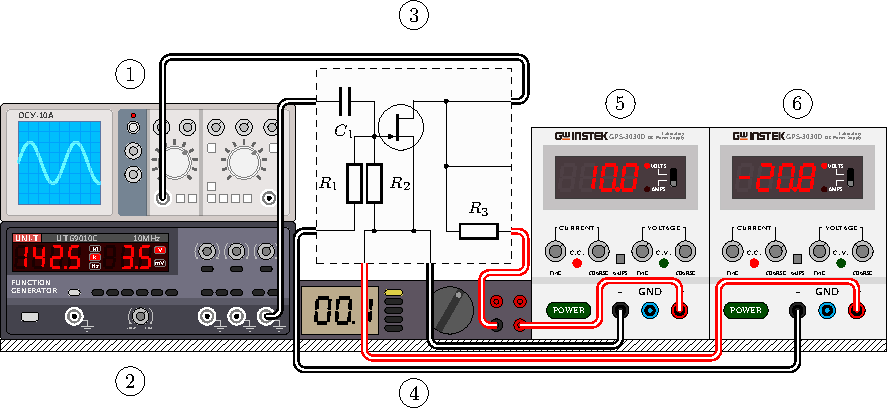
\includegraphics[width=\textwidth]{fig/view}
	\vspace{-1em}
	\caption{Лабораторная установка. 1 -- осциллограф ОСУ-10А, 2 -- генератор сигналов UNI-T UTG9010C, 3 -- измерительный модуль, подключенный в режиме усилителя входного сигнала, 4 -- мультиметр APPA-201N, 5,6 -- источники питания GPS-3030D (в принципиальной схеме -- $E_2$, $E_1$).}
	\label{fig:1}
\end{figure}

\newpage

\section{Измерение статических характеристик}

Для измерения статических характеристик измерительный модуль подключается по схеме, представленной на рис. \ref{fig:chem1}.

\begin{figure}[H]
	\centering
	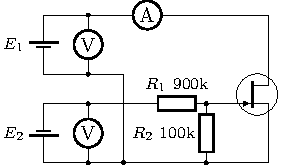
\includegraphics[scale=1.75]{fig/chem1}
	\caption{Принципиальная схема}
	\label{fig:chem1}
\end{figure}

\subsection{Переходные характеристики}
Измерено семейство переходных характеристик при различных фиксированных напряжениях на стоке.

\begin{figure}[H]
	\centering
	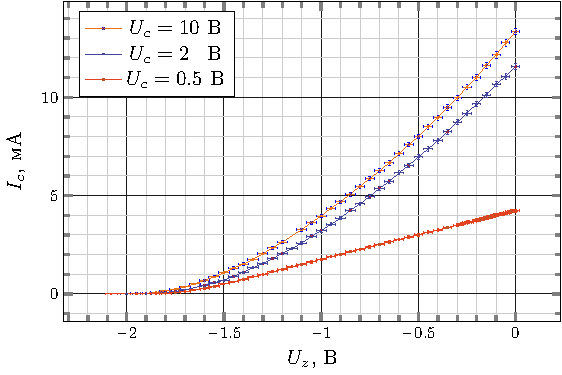
\includegraphics[scale=1.5]{fig/icuz.pdf}
	\vspace{-1em}
	\caption{Семейство переходных характеристик}
	\label{fig:2}
\end{figure}

При построении графиков учитывались инструментальные погрешности:
\begin{equation}
 \Delta U_z= \frac{1}{10} \Delta E_2 = \frac{1}{10}(0.005\cdot E_2+0.2) \text{ В}, \qquad
 \Delta I_c= (0.01\cdot I_c+0.02) \text{ мА}
\end{equation}

По обработанным данным рассчитана крутизна переходных характеристик. Для этого линейные участки характеристик аппроксимировались прямой с помощью MatLab:
\begin{equation}
\begin{aligned}
	S_{10}=\pdv{I_c}{U_z}\bigg|_{U_c=10\text{ В}}&=(10.4\pm0.15) \text{ кОм}^{-1},
	\\
	S_{2}=\pdv{I_c}{U_z}\bigg|_{U_c=2\text{ В}}&=(8.5\pm0.11)\text{ кОм}^{-1},
	\\
	S_{0.5}=\pdv{I_c}{U_z}\bigg|_{U_c=0.5\text{ В}}&=(2.5\pm0.09)\text{ кОм}^{-1}.
\end{aligned}
\end{equation}
Здесь в качестве ошибки принято среднеквадратичное отклонение аппроксимации. 

\subsection{Выходные характеристики} 
Проведены измерения выходных характеристик $I_c(U_c)$ при фиксированных значениях напряжения между затвором и истоком $U_z=0.1\cdot E_2$.

\begin{figure}[H]
	\centering
	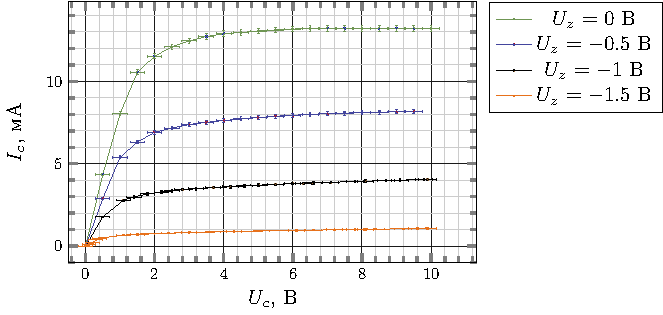
\includegraphics[scale=1.5]{fig/icuc.pdf}
	\vspace{-1em}
	\caption{Семейство выходных характеристик}
	\label{fig:2}
\end{figure}

На семействе выходных характеристик можно проследить наличие двух режимов: \textit{линейного} (омического), когда ток в канале растет почти прямо пропорционально напряжению на канале, и \textit{насыщения} -- когда ток почти перестает зависеть от напряжения на канале.


\section{Изучение режимов работы транзистора}

Включив измерительный модуль в режиме усиления сигнала (см. рис. \ref{fig:chem2}) измерили напряжение отсечки ($U_z=2.08$ В, при этом $I_c=0$). Затем подали на вход усилителя с генератора гармонический сигнал с размахом 0.146 В, частотой 45.07 кГц, а на сток транзистора подали постоянное напряжение $U_c=10$ В.


\begin{figure}[H]
	\centering
	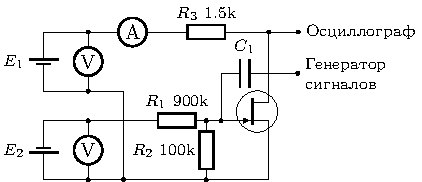
\includegraphics[scale=1.75]{fig/chem2}
	\caption{Принципиальная схема}
	\label{fig:chem2}
\end{figure}

\begin{figure}[H]
	\centering
	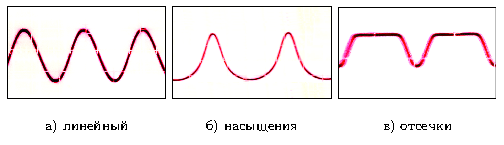
\includegraphics[width=\textwidth]{fig/osci}
	\vspace{-2em}
	\caption{Режимы работы транзистора}
	\label{fig:osci}
\end{figure}

Изменяя далее напряжение на затворе, получили:
\begin{itemize}
	\item Линейный режим при $U_z=0.37$ В, $U_c=0.2$ В
	\item Режим насыщения при $U_z=0.96$ В, $U_c=4.5$ В
	\item Режим отсечки при $U_z=2.08$ В, $U_c=10$ В
\end{itemize}
Осциллограммы выходного сигнала в трех режимах приведены на рис. \ref{fig:osci}.


% При напряжении E2=20.8в  (U_z=2.08в) наблюдается режим отсечки, ток I_c=0.00mA;
% На осциллографе, убирая постоянную сост., измерили напряжение сток-исток Uc=10в (две кл, 5в на кл).
% Сфотали осциллограмму.


% При напряжении E2=9.7в наблюдается режим насыщения, при этом ток I_c=3.84mA, напряжение сток-исток Uc=4.5в (4.5 кл, 1в на кл).
% Сфотали осциллограмму.


% При напряжении E2=3.7в наблюдается линейный режим, при этом ток I_c=6.19mA, напряжение сток-исток Uc=0.2в (2 кл, 0.1в на кл).
% Сфотали осциллограмму.


\section{Измерение коэффициента усиления}
Включив измерительный модуль в режиме однокаскадного усилителя с общим истоком в линейном режиме ($E_1=5$ В, $U_z=0.64$ В, $I_c=5.72$ мА) и подавая с генератора гармонический сигнал с размахом $0.145$ В и частотой в диапазоне 0.1 --- $10^7$ Гц, сняли АЧХ усилителя:
\begin{figure}[H]
	\centering
	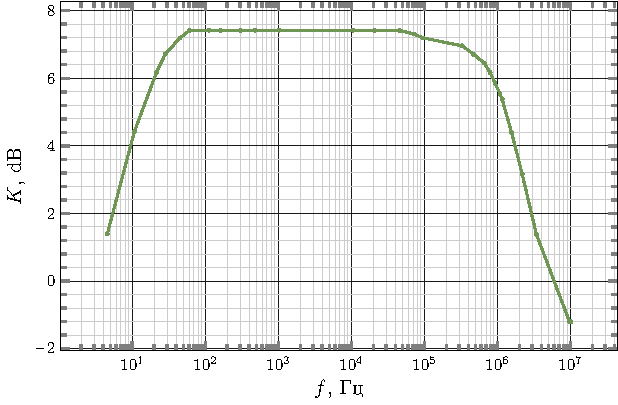
\includegraphics[scale=1.5]{fig/k_from_f.pdf}
	\vspace{-1em}
	% \caption{}
	\label{fig:arf}
\end{figure}

Предельная частота усиления без искажений по амплитуде -- 45 кГц в области высоких частот и 60 Гц -- в области низких. Частоты среза 10 Гц и 2 мГц (на частотах среза усиление падает вдвое по сравнению с полосой безискажательного пропускания).

% Собрали вторую схему, вошли в линейный режим (E1=10в, U_z=0.64в, I_c=5.72mA). Подали синус 145mV. АЧХ в файле ex8.tsv.
% На частоте ~ 2 мГц усиление падает ~ в "e" раз.
% и
\vspace{-1em}
\section{Измерение времен переключения}
Включив измерительный модуль в режиме однокаскадного усилителя с общим истоком в линейном режиме, выставив напряжение отсечки на затворе, подали с генератора сигналов меандр с амплитудой 3.5 В на частоте 142.5 кГц.

На осциллографе, который подключён к выходу усилителя, при этом наблюдается периодический сигнал, отвечающий переходу транзистора из режима отсечки в режим насыщения при приходе фронта меандра.

Измеряя на осциллографе ширину заднего и переднего фронта, получаем времена переключения $t_\uparrow$, $t_\downarrow$. 

\begin{figure}[H]
	\centering
	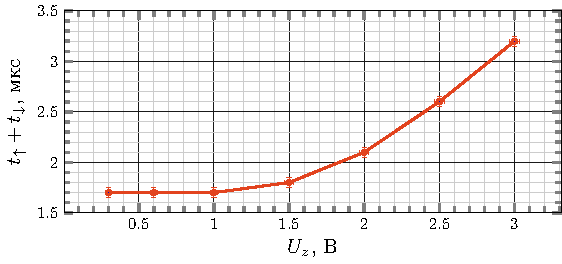
\includegraphics[scale=1.5]{fig/t_from_uz.pdf}
	\vspace{-1em}
	% \caption{}
	\label{fig:tfuz}
\end{figure}
Меняя напряжение на затворе, сняли зависимость времени переключения транзистора из отсечки в насыщение и обратно (см. рис. выше).

Максимальное суммарное время переключений  3.2 мкс, что дает предельную частоту 1.92 мГц. Это вполне согласуется с результатами предыдущего эксперимента.

% Однако,когда предельная частота транзистора станет сравнима с частотой сигнала, искажения сигнала неизбежны.


\vspace{-1em}
\addcontentsline{toc}{section}{Заключение}
\section*{Заключение}
В настоящей работе мы изучили принципы работы полевого транзистора, различные режимы работы (отсечка, насыщение, линейный), сняли семейства переходных и выходных статических характеристик, рассчитали крутизну переходных характеристик. Сняли АЧХ усилителя по схеме  с общим истоком, а также времена переключения транзистора.

% \newpage
\begin{thebibliography}{}
  \bibitem{orlov} Орлов И.\,Я., Односевцев В.\,А. и др. Основы радиоэлектроники: учебное пособие. -- Нижний Новгород: Нижегородский государственный университет им. Н.И. Лобачевского, 2011. -- 169 с.
  
  \bibitem{met} Битюрин\,\,Ю.\,А. и др. Измерение статических характеристик полевого транзистора. Н.Новгород: ННГУ, 2003. -- 30 с.
  
  % \bibitem{lit3} Ландау Л.Д., Лифшиц Е.М. Любой том. М.: Физматлит, 2003.
\end{thebibliography}

\end{document}